\chapter{Testování}\label{testovani}
% Nedílnou součástí vývoje softwaru je testování. Testování bylo rozděleno do dvou vrstev. Základní vrstvou jsou unit testy. Pro tvorbu těchto testů byl použit framework JUnit 5. Druhou vrstvou jsou integrační testy, které jsou implementovány pomoci funkcionality, kterou poskytuje framework Spring.
Testování je nedílnou součástí implementace libovolného softwaru a je jeho velice důležitou častí. V rámci této bakalářské práce testům byla věnovaná řádná pozornost, proto bylo vyřešeno věnovat testům samostatnou kapitolu. V teto kapitole bude popsán proces testování, doplňující funkcionalita, zjednodušující proces testování. Také bude popsáno pokrytí kódů testy.
\section{Tagy}\label{testovani:tagy}
    Tagy už byly zmíněné v sekci \ref{navrh:testovani}, proto v teto sekci ihned se zanoříme do podrobného popisu implementace. 
    
    Na začátku je potřeba popsat chování tagů a proč je potřebujeme. Tagy označují jednotlivé testy nebo celé testovací třídy pomocí obyčejného textového řetězce (viz. obrázek \ref{code:tag-junit-5}). Obsah řetězce může být libovolný. Za účelem pohodlnějšího využití testu byly zvolené tagy, které popisuje konkretní aspekt jeho chování. Například, pomalý test nebo integrační test. Při spouštěni testů pomocí frameworku JUnit můžeme definovat testy které bychom potřebovali spustit pomocí předem definovaných tagů. Stejného výsledku bychom mohli dosáhnout pomocí třídění testů do různých složek, ale podstatný rozdíl mezi těmito postupy je v tom, že jeden test může mít několik tagů zároveň. Například test může být anotován jako pomalý integrační test a zároveň jako pomalý test, protože využívá databázi. Takový výsledek je docela složitý při tříděni testů do různých složek.
    \begin{figure}
        \begin{minted}{java}
@Tags(
        Tag("integration_test")
)
        \end{minted}
        \caption{Příklad tagu frameworku JUnit 5} 
        \label{code:tag-junit-5}
    \end{figure}
    
    Tagy jsou jenom textové řetězce, proto je docela očividně, že je velká pravděpodobnost překlepu při implementací velkého počtu testů\footnote{na moment odevzdání bakalářské práci bylo implementováno 126 testů v 25 třídách}. Proto bylo vyřešeno definovat vlastní anotace s předem definovanými tagy. Ve výsledku byly implementovány 4 tagy:
    \begin{itemize}
            \item \textit{IntergationTest}, který má tag obsahující text \enquote{integration\_test}
            \item \textit{SecurityTest}, který má tag obsahující text \enquote{security\_test}
            \item \textit{SlowTest}, který má tag obsahující text \enquote{slow\_test}
            \item \textit{UnitTest}, který má tag obsahující text \enquote{unit\_test}
    \end{itemize}
    
    Anotace mají stejnou implementací a liší se jenom pomocí textu uvnitř tagů. Kotlin poskytuje funkcionalitu pro vytváření vlastních anotací, proto byla využita vestavěna třída anotace (viz. obrázek \ref{code:annotation-class}). Anotace jsou implementovány takovým způsobem, že pomocí ně je možné anotovat ne jenom testové metody, ale i celé třídy. Pak anotace se aplikuje na každý test, který obsahuje anotovaná třída. Také je možné anotovat i jiné anotace.
    \begin{figure}
        \begin{minted}{java}
/**
 * Specifies test as a Integration test.
 */
@Target(allowedTargets = [
        AnnotationTarget.FUNCTION,
        AnnotationTarget.ANNOTATION_CLASS,
        AnnotationTarget.CLASS
])
@Retention(AnnotationRetention.RUNTIME)
@MustBeDocumented
@Tags(
        Tag("integration_test")
)
annotation class IntegrationTest
        \end{minted}
        \caption{Příklad třídy Anotace zaměňující tag s textem \enquote{integration\_test}} 
        \label{code:annotation-class}
    \end{figure}
    % Během vývoje velkých projektů zpouštění testů je významným problémem pro programátory. 
    % Framework JUnit 5 poskytuje možnost označovat metody a třídy pomocí tagu.
\section{Zobrazování testů}\label{testovani:zobrazovani}
    % TODO v pripade ze pobezi testy pres IDEA. Pres terminal nefunguje CamelCaseGenerator
    Správné a pochopitelné zobrazování názvů testu mnohem zjednodušuje proces testování. Proto před začátkem implementaci testů byly navrženo pravidlo pro zobrazování testu. Název testu má obsahovat v názvu stručný popis toho, co by měl test otestovat. 
    
    \begin{figure}\centering
	   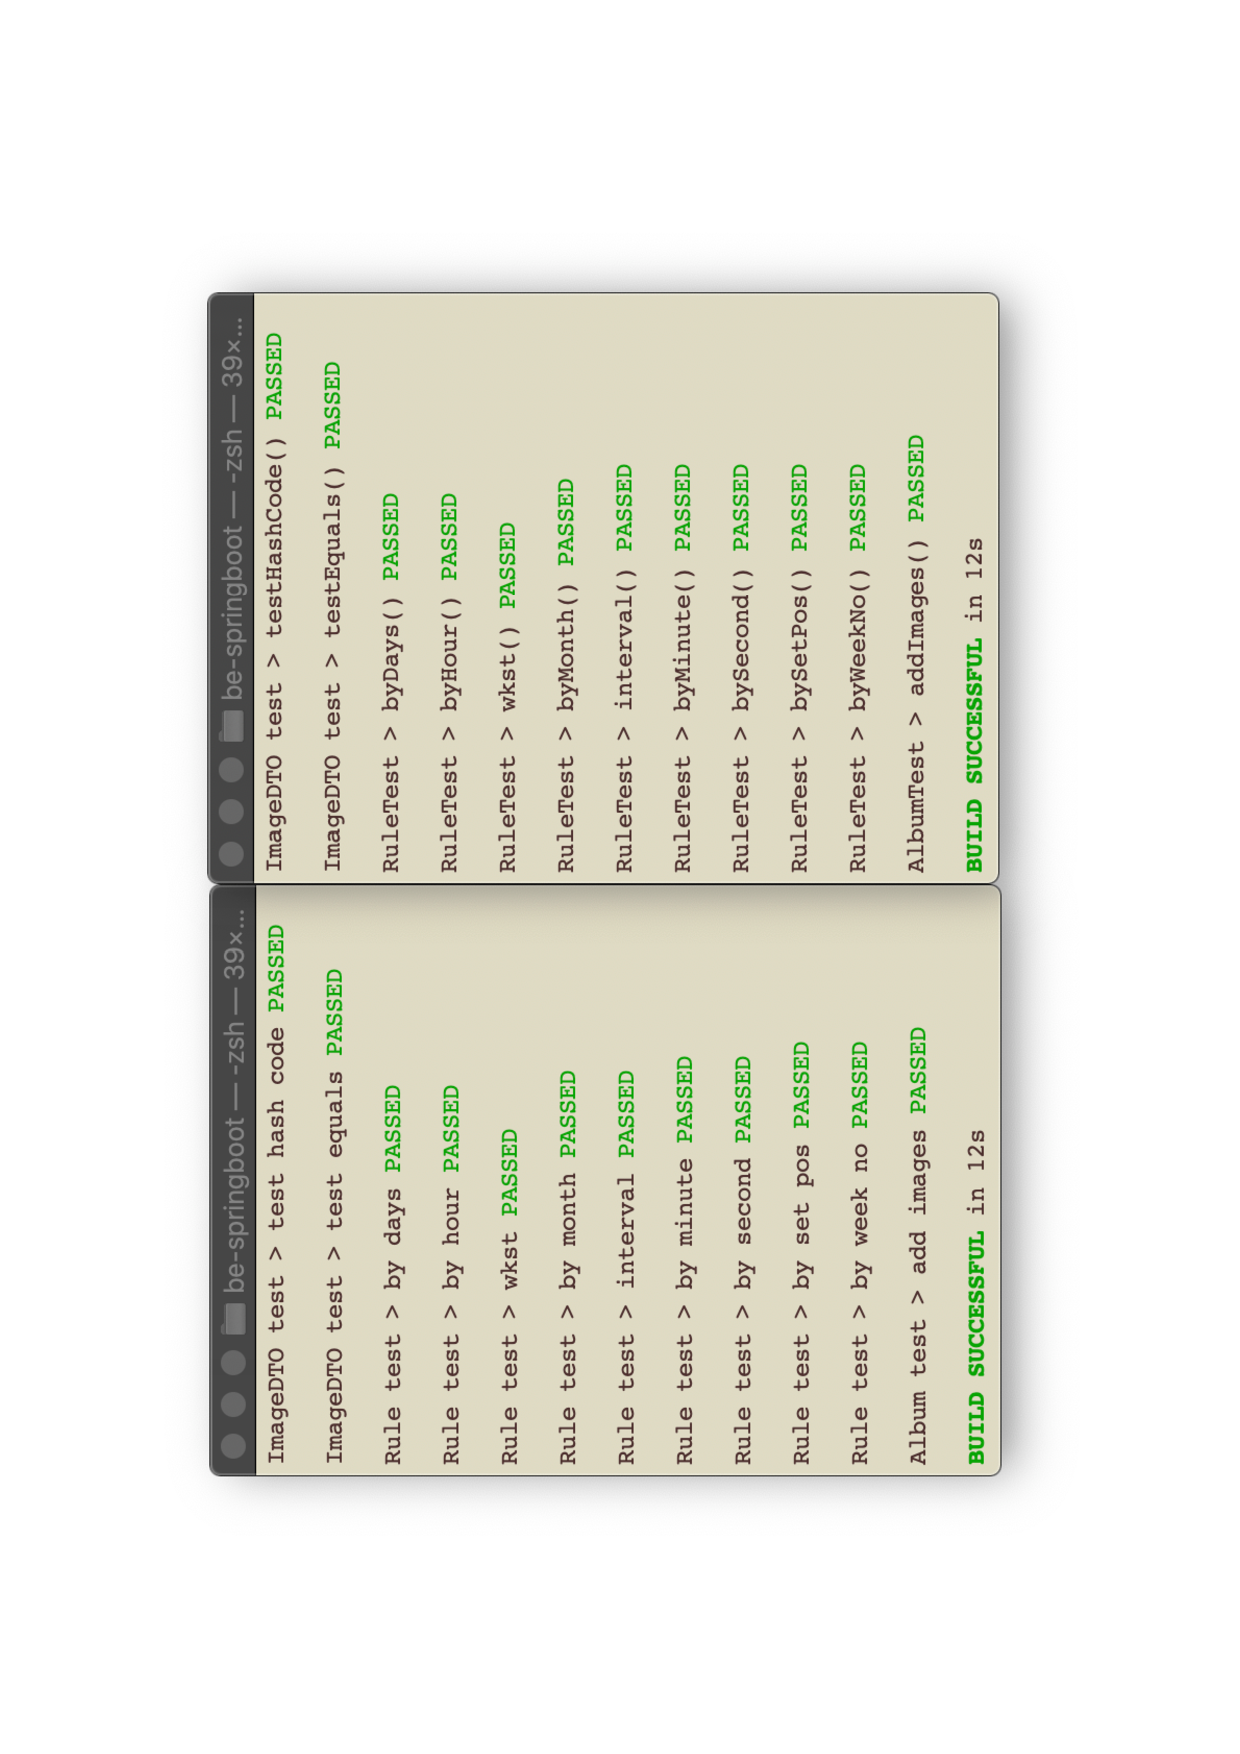
\includegraphics[angle=-90, width=1.0\textwidth]{pdfs/pretty-tests-comparison}
	   \caption[Srovnaní zobrazováni kódu]{Příklad vypisování testů pomocí generátoru a bez}\label{image:pretty-tests-comparison}
    \end{figure}
    Pro čitelnější zobrazování byl implementován generátor transformující jméno testu nebo jméno třídy do čitelnější podoby (viz. obrázek \ref{image:pretty-tests-comparison}). Princip fingování je založen na překladu názvu ve velbloudí notace na obyčejný text s mezerami. Také výsledné názvy testu a tříd neobsahují žádné zbytečné symboly\footnote{například, za zbytečné symboly jsou považovány prázdné závorky na konci názvu metody} Pro pohodlné využiti generátoru byla implementována anotace, která je aplikovatelná na třídy. Anotace aktivuje generátor pro všechny testy, které třída obsahuje. 
    
    V případě, že název metody obsahuje text, který by se neměl korektně transformovat, potřebujeme použit anotaci \textit{DisplayName} a v závorkách teto anotaci uvést text, který by měl být zobrazen. Tento název přepisuje výsledek generátoru, proto tato anotace může být použita ve třídě, která má anotaci generátoru. Příkladem takového nevhodného názvu může být třída se jménem \enquote{ImageDTO}, která bude přeložena na \enquote{Image d t o}, což zjevně není požadováným výsledkem.
%     \begin{figure}
%         \begin{minted}{java}
% class CamelCaseGenerator : DisplayNameGenerator.Standard() {
%     override fun generateDisplayNameForNestedClass(
%             nestedClass: Class<*>?): String {
%         return toCamelCase(super.generateDisplayNameForNestedClass(nestedClass))
%     }

%     override fun generateDisplayNameForMethod(
%             testClass: Class<*>?,
%             testMethod: Method?): String {
%         return toCamelCase(testMethod!!.name)
%     }

%     override fun generateDisplayNameForClass(testClass: Class<*>?): String {
%         return toCamelCase(super.generateDisplayNameForClass(testClass))
%     }

%     private fun toCamelCase(name: String): String {
%         val result = StringBuilder()
%         result.append(name.ifEmpty { return "" }.first())
%         for (char in name.substring(1)) {
%             if (Character.isUpperCase(char)) {
%                 result.append(' ')
%                 result.append(Character.toLowerCase(char))
%             } else {
%                 result.append(char)
%             }
%         }
%         return result.toString()
%     }

% }
%         \end{minted}
%         \caption{Třída transformující jména metod a tříd do čítelné podoby} 
%         \label{code:DNG}
%     \end{figure}
    
\section{Unit testy}\label{testovani:unit}
    TODO Unit testy jsou zaměřené na otestování samostatně testovatelných metod a tříd.
    
\section{Integrační testy}\label{testovani:intergacni}
    TODO Integrační testy zaměřené na ověření správné komunikace mezi komponentami aplikace.
    
\section{Samostatný profil pro testování}

    Testovaní aplikace vyžaduje vlastní nastavení, proto byl vytvořen samostatný profil, který odděluje testovací nastavení od nastavení produkce a vývoje. Profil má vlastní konfigurační soubor (\textit{application-test.properties}), obsahující nastavění databáze.
    
    Pro testování byla  využita stejná databáze jako i pro proces vývoje, za účelem kompletního a rychlého testování serveru. Databáze umožňuje rychle zničit a vytvořit tab, což nám umožňuje rychle zničit kontext aplikace mezi integračními testy.
    
    Také profil pro testování má vlastní implementaci pro \textit{UserDetailsService}\footnote{Základní rozhraní, které framework Spring využívá pro načítaní informace o uživateli}, obsahující tří implicitní uživatele:
    \begin{itemize}
            \item \textit{root}, vlastnící role \enquote{ROLE\_USER} a \enquote{ROLE\_ROOT} 
            \item \textit{userEmail}, vlastnící role \enquote{ROLE\_USER}
            \item \textit{user2Email}, vlastnící role \enquote{ROLE\_USER}
    \end{itemize}
    Tyto implicitní uživatel jsou využité v integračních testech pro spouštění požadavků (\textit{requestů}) přes instanci MocMvc. Podrobněji integrační testy byly popsány v sekci \ref{testovani:intergacni}.
    
\section{Pokrytí kódu testy}\label{testovani:pokryti}
    % TODO V teto sekci je uveden popis provedéní analýzy pokrýtí kódu testy.
    V teto sekci bude popsáno pokrytí kódů testy a uvedeny statistiky. Za účelem zvýšení pravděpodobnosti provedené analýzy testování, byly využité speciální nástroje pro zhodnocení pokrýti kódů.
    \subsection{JaCoCo}
    Prvním nástrojem, který byl využit pro analýzu testů, je Jacoco. Tento nástroj byl podrobně popsán v sekci \ref{resere:testovani:jacoco}. V teto sekci uvedeme jenom proces analýzy a její výsledky.
    
    JaCoCo vyžaduje implementování vlastního \textit{tasku}\footnote{Konfigurovatelný úkol pro buildovácí systém Gradle. Například, \textit{test} nebo \textit{build}}(\textit{jacocoTestReport}) v Gradle. Generování výsledků závisí na spouštění klasického úkolu \textit{test} od Gradle. 
    
    Generování výsledků pokrýti testu bylo využito jako nápověda pro identifikování důležitého kódu nepokrytého testy. Proto úkol \textit{jacocoTestReport} byl spouštěn několikrát. Podle poslední verze výsledku, která byla spouštěna pro poslední verzi aplikace, 85 \% instrukcí jsou pokryté testy. Podrobnou informaci se můžete dozvědět v příloze \ref{dodatek:code-coverage}.
    % vestaveny junit engine v IntelifIDEA prestal fingovat po dosazeni velkeho poctu testu
    \subsection{IntelliJ IDEA}
    Druhým testovacím nástrojem, který byl využit pro zjištění pokrytí kódů testy, je InteliJ IDEA. Podrobněji tento nástroj byl popsán v sekci \ref{resere:testovani:intellij-idea}. 
    
    Tento nástroj také byl využit jako pomocný nástroj při implementaci testů. V teto sekci budou uvedený jenom výsledky posledního spouštění pro poslední verzi aplikace. Kompletní informaci o výsledcích najdete v příloze \ref{dodatek:code-coverage}.
    
    IntelliJ IDEA poskytuje trochu jinou informaci o pokrytí kódů než nástroj JaCoCo. Podle výsledku jsou pokryté testy:
    \begin{itemize}
            \item 72,6 \% tříd
            \item 90,1 \% metod
            \item 89,3 \% řádek kódů
    \end{itemize}
    